\documentclass[a4paper,10pt]{article}
\usepackage{amsmath}
\usepackage{amsfonts}
\usepackage{graphicx}
\usepackage{color}
\usepackage{graphicx}

\title{CS5321 Numerical Optimization Homework 2}
\author{Due Dec 2}
\date{}
\begin{document}
\maketitle
\begin{enumerate}
 \item (20\%) Check out  the TRUST-REGION NEWTON- LANCZOS METHOD in Section 7.1 in the .  What kind of problem it wants to solve? and how the Lanczos method solves it. 

\item (20\%) Check out section 8.2 in the deep learning textbook.  Give a summary about the major challenges in neural network optimization.

\item (10\%)  Let $J$ be an $m\times n$ matrix, $m\ge n$.  Show that $J$ has full column rank if and only if $J^TJ$ is positive definite.
 


\item (30\%) Simplex method (the algorithm is shown in Figure 2): Consider the following linear program:
    $$\begin{array}{lll}
        \max_{x_1,x_2} & z=8x_1+5x_2 \\
        \mbox{s.t. } & 2x_1 + x_2 \le 1000  \\
         & 3x_1 + 4x_2 \le 2400   \\
         & x_1 + x_2 \le 700   \\
         & x_1 - x_2 \le 350   \\
         & x_1, x_2 \ge 0
      \end{array}$$
      \begin{enumerate}
    \item Transform it to the standard form. 
    \item Suppose the initial guess is $(0,0)$.  Use the simplex method to solve this problem. In each iteration, show
      \begin{itemize}
    \item Basic variables and non-basic variables, and their values.
    \item Pricing vector.
    \item Search direction.
    \item Ratio test result.
    \end{itemize}
    \end{enumerate}

\item (20\%) Farkas lemma: Let $A$ be an $m\times n$ matrix and $\vec{b}$ be an $m$ vector.
Prove that exact one of the following two statements is true:
\begin{enumerate}
\item There exists a $\vec{x}\in \mathbb{R}^n$ such that $A\vec{x} =\vec{b}$ and $\vec{x}\ge0$.
\item There exists a $\vec{y}\in\mathbb{R}^m$ such that $A^T\vec{y}\ge 0$ and $\vec{b}^T\vec{y}<0$.
\end{enumerate}
(Hint: prove if (a) is true, then (b) cannot be true, and vice versa.)

\end{enumerate}

\begin{figure}
\begin{tabular}{cc}
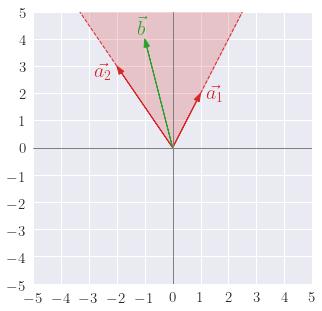
\includegraphics[width=.5\textwidth]{farkas1.png} & 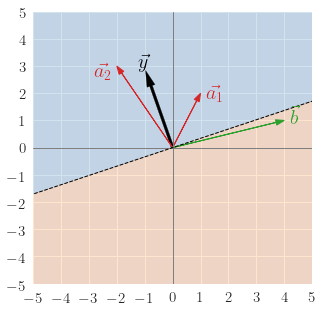
\includegraphics[width=.5\textwidth]{farkas2.png} \\
case (a) & case (b) \\
\end{tabular}
\caption{Two cases of Farkas Lemma.}
\end{figure}

\fbox{
 \parbox{\textwidth}{
Farkas's Lemma (1902) plays an important role in the proof of the KKT condition. The most critical part in the proof of the KKT condition is to show that the Lagrange multiplier $\vec{\lambda}^*\ge 0$ for inequality constraints. We can say if the LICQ condition is satisfied at $\vec{x}^*$, then any feasible direction $\vec{u}$ at $\vec{x}^*$ must have the following properties:
\begin{enumerate}
\item $\vec{u}^T\nabla f(\vec{x}^*) \ge 0$ since $\vec{x}^*$ is a local minimizer. 
(Otherwise, we find a feasible descent direction that decreases $f$.)
\item $\vec{u}^T\nabla c_i(\vec{x}^*) = 0$ for equality constraints, $c_i = 0$.
\item $\vec{u}^T\nabla c_i(\vec{x}^*) \ge 0$ for inequality constraints, $c_i \ge 0$.
\end{enumerate}
Here is how Farkas Lemma enters the theme. Let $\vec{b}$ be $\nabla f(\vec{x}^*)$, $\vec{y}$ be $\vec{u}$ (any feasible direction at $\vec{x}^*$), the columns of $A$ be $\nabla c_i(\vec{x}^*)$). Since no such $\vec{u}$ exists, according to the properties of $\vec{y}$, statement (a) must hold. The vector $\vec{x}$ in (a) corresponds to $\vec{\lambda}^*$, which just gives us the desired result of the KKT condition.
}}

\begin{figure}[hb]
  \begin{center}
  \begin{tabular}{cp{.2in}l}
    \hline \hline \\[0pt]
  (1) & \multicolumn{2}{l}{Given a basic feasible point $\vec{x}_0$ and the corresponding index set}\\
   & \multicolumn{2}{l}{ $\mathcal{B}_0$ and $\mathcal{N}_0$.} \\
  (2) & \multicolumn{2}{l}{For $k=0,1,\ldots$} \\
  (3) & & Let $B_k=A(:,\mathcal{B}_k), N_k=A(:,\mathcal{N}_k)$, $\vec{x}_B=\vec{x}_k(\mathcal{B}_k),
  \vec{x}_N=\vec{x}_k(\mathcal{N}_k)$, \\
     &  & and $\vec{c}_B=\vec{c}_k(\mathcal{B}_k), \vec{c}_N=\vec{c}_k(\mathcal{N}_k)$.\\
  (4) & & Compute $\vec{s}_k=\vec{c}_N-N_k^TB_k^{-1}\vec{c}_B$  \mbox{\color{blue}(pricing)} \\
  (5) & & If $\vec{s}_k\ge 0$, return the solution $\vec{x}_k$. \mbox{\color{blue}(found optimal solution)} \\
  (6) & & Select $q_k\in\mathcal{N}_k$ such that $\vec{s}_k(i_q)<0$, \\
    & & where $i_q$ is the index of $q_k$ in $\mathcal{N}_k$\\
  (7) & & Compute $\vec{d}_k=B^{-1}_kA_k(:,q_k)$. \mbox{\color{blue}(search direction)} \\
  (8) & & If $\vec{d}_k\le 0$, return \verb"unbounded". \mbox{\color{blue}(unbounded case)} \\
  (9) & & Compute $\displaystyle [\gamma_k, i_p] = \min_{i,\vec{d}_k(i)>0}\frac{\vec{x}_B(i)}{\vec{d}_k(i)}$ \mbox{\color{blue}(ratio test)}\\
  &&\mbox{\color{blue}(The first return value is the minimum ratio;}\\
  &&\mbox{\color{blue} the second return value
  is the index of the minimum ratio.)} \\
  (10) & & $\displaystyle x_{k+1}\left(
                     \begin{array}{c}
                       \mathcal{B} \\
                       \mathcal{N} \\
                     \end{array}
                   \right) =  \left(
                     \begin{array}{c}
                       \vec{x}_B \\
                       \vec{x}_N \\
                     \end{array}
                   \right) + \gamma_k \left(
                     \begin{array}{c}
                       -\vec{d}_k \\
                       \vec{e}_{i_q} \\
                     \end{array}
                   \right)$ \\
  &&\mbox{\color{blue}($\vec{e}_{i_q}=(0,\ldots,1,\ldots,0)^T$ is a unit vector with $i_q$th element 1.)}\\
  (11) &&Let the $i_p$th element in $\mathcal{B}$ be $p_k$. \mbox{\color{blue}(pivoting)} \\
       & & $\mathcal{B}_{k+1}=(\mathcal{B}_k-\{p_k\})\cup\{q_k\}$,  $\mathcal{N}_{k+1}=(\mathcal{N}_k-\{q_k\})\cup\{p_k\}$  \\[10pt]
  \hline \hline
  \end{tabular}
  \end{center}
  \caption{The simplex method for solving (minimization) linear programming}\label{}
\end{figure}


\end{document}
